\documentclass[a4paper,11pt]{article}

\usepackage{fontspec}
\usepackage[ngerman]{babel}
\usepackage{graphicx}
\usepackage{eso-pic}
\usepackage{tabularx}
\usepackage{stackengine}
\usepackage{ragged2e}
\usepackage{url}
\usepackage{gensymb}    %grad zeichen
\usepackage{hyperref}
\usepackage{microtype}
\usepackage{unicode-math}
\setmathfont{Latin Modern Math}     % gegen Warnung wegen Arial Schriftart (ihr fehlt der Mathepart)
\usepackage[left=3cm, right=5cm, top=1.5cm, bottom=2cm]{geometry}
\usepackage{setspace}
\onehalfspacing                 % Zeilenabstand
\setmainfont{Arial}

\emergencystretch=2em  %kein überstehender Text (hoffentlich)

\usepackage{parskip}         % für eindeutige Absätze
\usepackage[all]{nowidow}    % gegen verwaiste Zeilen

\usepackage{titlesec}        %strich unter section
\titleformat{\section}{\normalfont\Large\bfseries}{\thesection}{1em}{}[\titlerule\vspace{0.5cm}]


\author{}
\date{}
\title{{\fontsize{26pt}{30pt}\selectfont Seminarfach} \\[3cm] {\fontsize{30pt}{40pt}\selectfont Facharbeit}}


\newcommand{\StartBackground}{
\newgeometry{top=6.2cm,bottom=1.5cm,left=4cm,right=2cm}
\AddToShipoutPictureBG{
\put(0,0){
\parbox[b][\paperheight]{\paperwidth}{
\vfill
\centering

\includegraphics[width=\paperwidth,height=\paperheight]{../Background.png}
\vfill}}}}
\newcommand{\StopBackground}{\newpage\restoregeometry\ClearShipoutPictureBG}

\pagestyle{empty}
\pagenumbering{gobble}


% label und section zusammen (pure Faulheit)

\newcommand{\mysection}[1]{\section{#1}\label{sec:#1}}
\newcommand{\mysubsection}[1]{\subsection{#1}\label{subsec:#1}}
\newcommand{\mysubsubsection}[1]{\subsubsection{#1}\label{subsubsec:#1}}




% Zitation

\usepackage{csquotes}

\usepackage[
    style=authoryear,
    backend=biber,
    natbib=true,
    maxcitenames=1,
    mincitenames=1,
    maxbibnames=3,
    minbibnames=3,
    citetracker=context,
    giveninits=true,
    uniquelist=false
]{biblatex}


\AtEveryCite{\renewbibmacro*{name:andothers}{}}

\DefineBibliographyStrings{ngerman}{andothers = {et\addabbrvspace al\adddot}}

\renewcommand*{\postnotedelim}{\addcolon\space}

\renewcommand*{\multicitedelim}{\addsemicolon\space}

\DeclareFieldFormat{postnote}{S.#1}

\DeclareFieldFormat[book,thesis]{title}{\mkbibemph{#1}}

\DeclareFieldFormat[article,inbook,incollection,inproceedings,inreference,online,report,misc]{title}{#1}

\DeclareDelimFormat{finalnamedelim}{\space/\space}

\DeclareDelimFormat{multinamedelim}{\space/\space}

\DeclareNameFormat{author}{\ifnum\value{listcount}=1
\nameparts{#1}
\usebibmacro{name:family-given}
{\namepartfamily}
{\namepartgiven}
{\namepartprefix}
{\namepartsuffix}
\else
\nameparts{#1}
\usebibmacro{name:given-family}
{\namepartfamily}
{\namepartgiven}
{\namepartprefix}
{\namepartsuffix}\fi\ifboolexpr{test {\ifnumcomp{\value{listcount}}{=}{\value{liststop}}}
and test {\ifmorenames}}{\ifnumgreater{\value{liststop}}{1}{\finalnamedelim}{}\usebibmacro{name:andothers}}{}}

\DeclareNameAlias{editor}{family-given}
\setlength{\bibhang}{1.25cm}
\setlength{\bibitemsep}{0.5\baselineskip}
\setlength{\bibparsep}{0pt}
\DefineBibliographyStrings{ngerman}{editor = {Hrsg\adddot},editors = {Hrsg\adddot}}
\DeclareLabeldate{\field{date}\field{year}}
\ExecuteBibliographyOptions{uniquename=false}
\DefineBibliographyStrings{ngerman}{urlseen = {Zugriff am}}
\renewcommand*{\bibfont}{\fontsize{11pt}{14pt}\selectfont}
\newcommand{\ebd}[1][]{\text{(ebd.\if\relax\detokenize{#1}\relax\else~S.#1\fi)}}
\AtBeginBibliography{\interlinepenalty=10000}
\AtEveryBibitem{\clearfield{doi}\clearfield{issn}}
\addbibresource{../Quellen/Quellen.bib}



%---------------------------------------------------------------------------------
% Titelseite / Benotung

\begin{document}
\justifying                 % => für Blocksatz
\StartBackground

\maketitle
\vspace{5cm}
\begin{table}[h!]
    \renewcommand{\arraystretch}{3}
    \begin{tabularx}{\textwidth}{>{\raggedright\arraybackslash}p{5cm}
                                 >{\raggedright\arraybackslash}X}
        \textbf{Thema:}&Entstehungsmechanismen und strukturelle Merkmale von Zentralbergen in Impaktkratern, Vulkanen und Äquatorialkämmen im Sonnensystem\\
        \textbf{Verfasser:}& Julian Luke Mawill Baden \\
        \textbf{Fachlehrkraft und Kursbezeichnung:}& Herr Ropeter , 13sf2\\
        \end{tabularx}
\end{table}


\newpage
\noindent\textbf{Gymnasium Mellendorf\\Fritz-Sennheiser-Platz 2\\30900 Wedemark}\\
Schuljahr:  2026/27\\

{\fontsize{26pt}{20pt}\selectfont\begin{center} Seminarfach \end{center}}

\noindent\rule{\linewidth}{0.5pt}

\begin{table}[h!]
    \renewcommand{\arraystretch}{2}
    \begin{tabularx}{\textwidth}{>{\raggedright\arraybackslash}p{4.5cm}
                                 >{\raggedright\arraybackslash}X}
        Verfasser:& Julian Luke Mawill Baden \\
        Thema:&Entstehungsmechanismen und strukturelle Merkmale von Zentralbergen in Impaktkratern, Vulkanen und Äquatorialkämmen im Sonnensystem\\
        Fachlehrkraft und Kursbezeichnung:& Herr Ropeter , 13sf2\\
        \end{tabularx}
\end{table}

\noindent\rule{\linewidth}{0.5pt}\\[0.5cm]
\textbf{Abgabetermin: 05.10.2026 zu Beginn der Seminarfachsitzung um 14 Uhr}\\[0.3cm]
\rule{\linewidth}{0.5pt}\\

\begin{tabular}{l  l}
    &\\
    \textbf{Benotung:}&\fbox{\rule[-1.5em]{0pt}{4em}\hspace{3cm}}\\
    &\\[0.3cm]
\end{tabular}\\


\phantom{y} \qquad \qquad Julian Luke Mawill Baden\\[1.2cm]


\hspace{1cm} \stackunder[4pt]{\rule{4.5cm}{0.6pt}}{\makebox[4.5cm]{Datum}}
\hspace{2cm} \stackunder[4pt]{\rule{5.5cm}{0.6pt}}{\makebox[5.5cm]{Unterschrift der Lehrkraft}}


\StopBackground



%---------------------------------------------------------------------------------
% Inhaltsverzeichnis


\normalsize

\pagestyle{plain}
\pagenumbering{Roman}
\setcounter{page}{1}

\tableofcontents
\newpage



%---------------------------------------------------------------------------------
% Inhalt

\onehalfspacing
\normalsize
\pagenumbering{arabic}






\section{Einführung}
















%---------------------------------------------------------------------------------
% Zentralberge


\mysection{Zentralberge}
\mysubsection{Was sind Zentralberge}

Zentralberge kommen in größeren Impaktkratern auf allen festen Himmelskörpern vor.
Es handelt sich um zentrale Erhöhungen in der Kratermitte,
die sich in der dritten Phase der Kraterentstehung formen (siehe Kapitel \ref{subsec:Entstehung}).

Ein anschauliches Beispiel für einen Krater mit Zentralberg ist der Tooting-Krater (siehe Abb.\ref{pic:tooting}).
Der auf dem Mars, in der Amazonis Planitia,
westlich des Olympus Mons, liegende Krater besitze einen Radius von 29~km und
einen $\sim$1100~m hohen Zentralberg \citep[1615, 1616, 1619]{Mouginis-Mark_2012}.
Das umliegende Terrain und das juge Alter des Kraters, macht exakte Tiefenmessungen möglich \ebd[1616].
so liegt der Kraterboden der südlichen Kraterhälfte $~\sim$1275~m unter dem umliegenden Terrain und
der nördliche Kraterboden auf $\sim$1080~m (siehe Abb.\ref{pic:tooting})\citep[1]{Mouginis-Mark_2015}.

Der Zentralberg des Tooting-Kraters liegt 119~m unterhalb der Kraterumgebung und
768~m unterhalb der durschnittlichen Randkamms des Kraters \ebd[].
Der Tooting-Krater zeichnet sich durch mehrere sekundäre Bergspitzen aus.
Die zentrale Spitze erreicht eine Höhe von 1110~m über dem Kraterboden \ebd[],
Die Sekundären Spitzen 149 und 147~m unterhalb dieser \citep[1619]{Mouginis-Mark_2012}.


\begin{center}
    \begin{figure}
        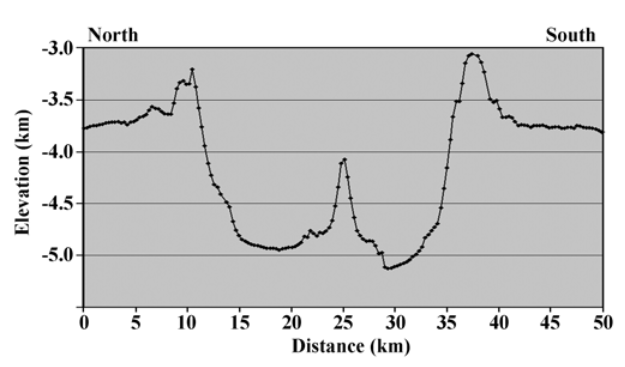
\includegraphics[width=0.55\textwidth]{../Quellen/Bilder/Tooting_querschnitt.png}
        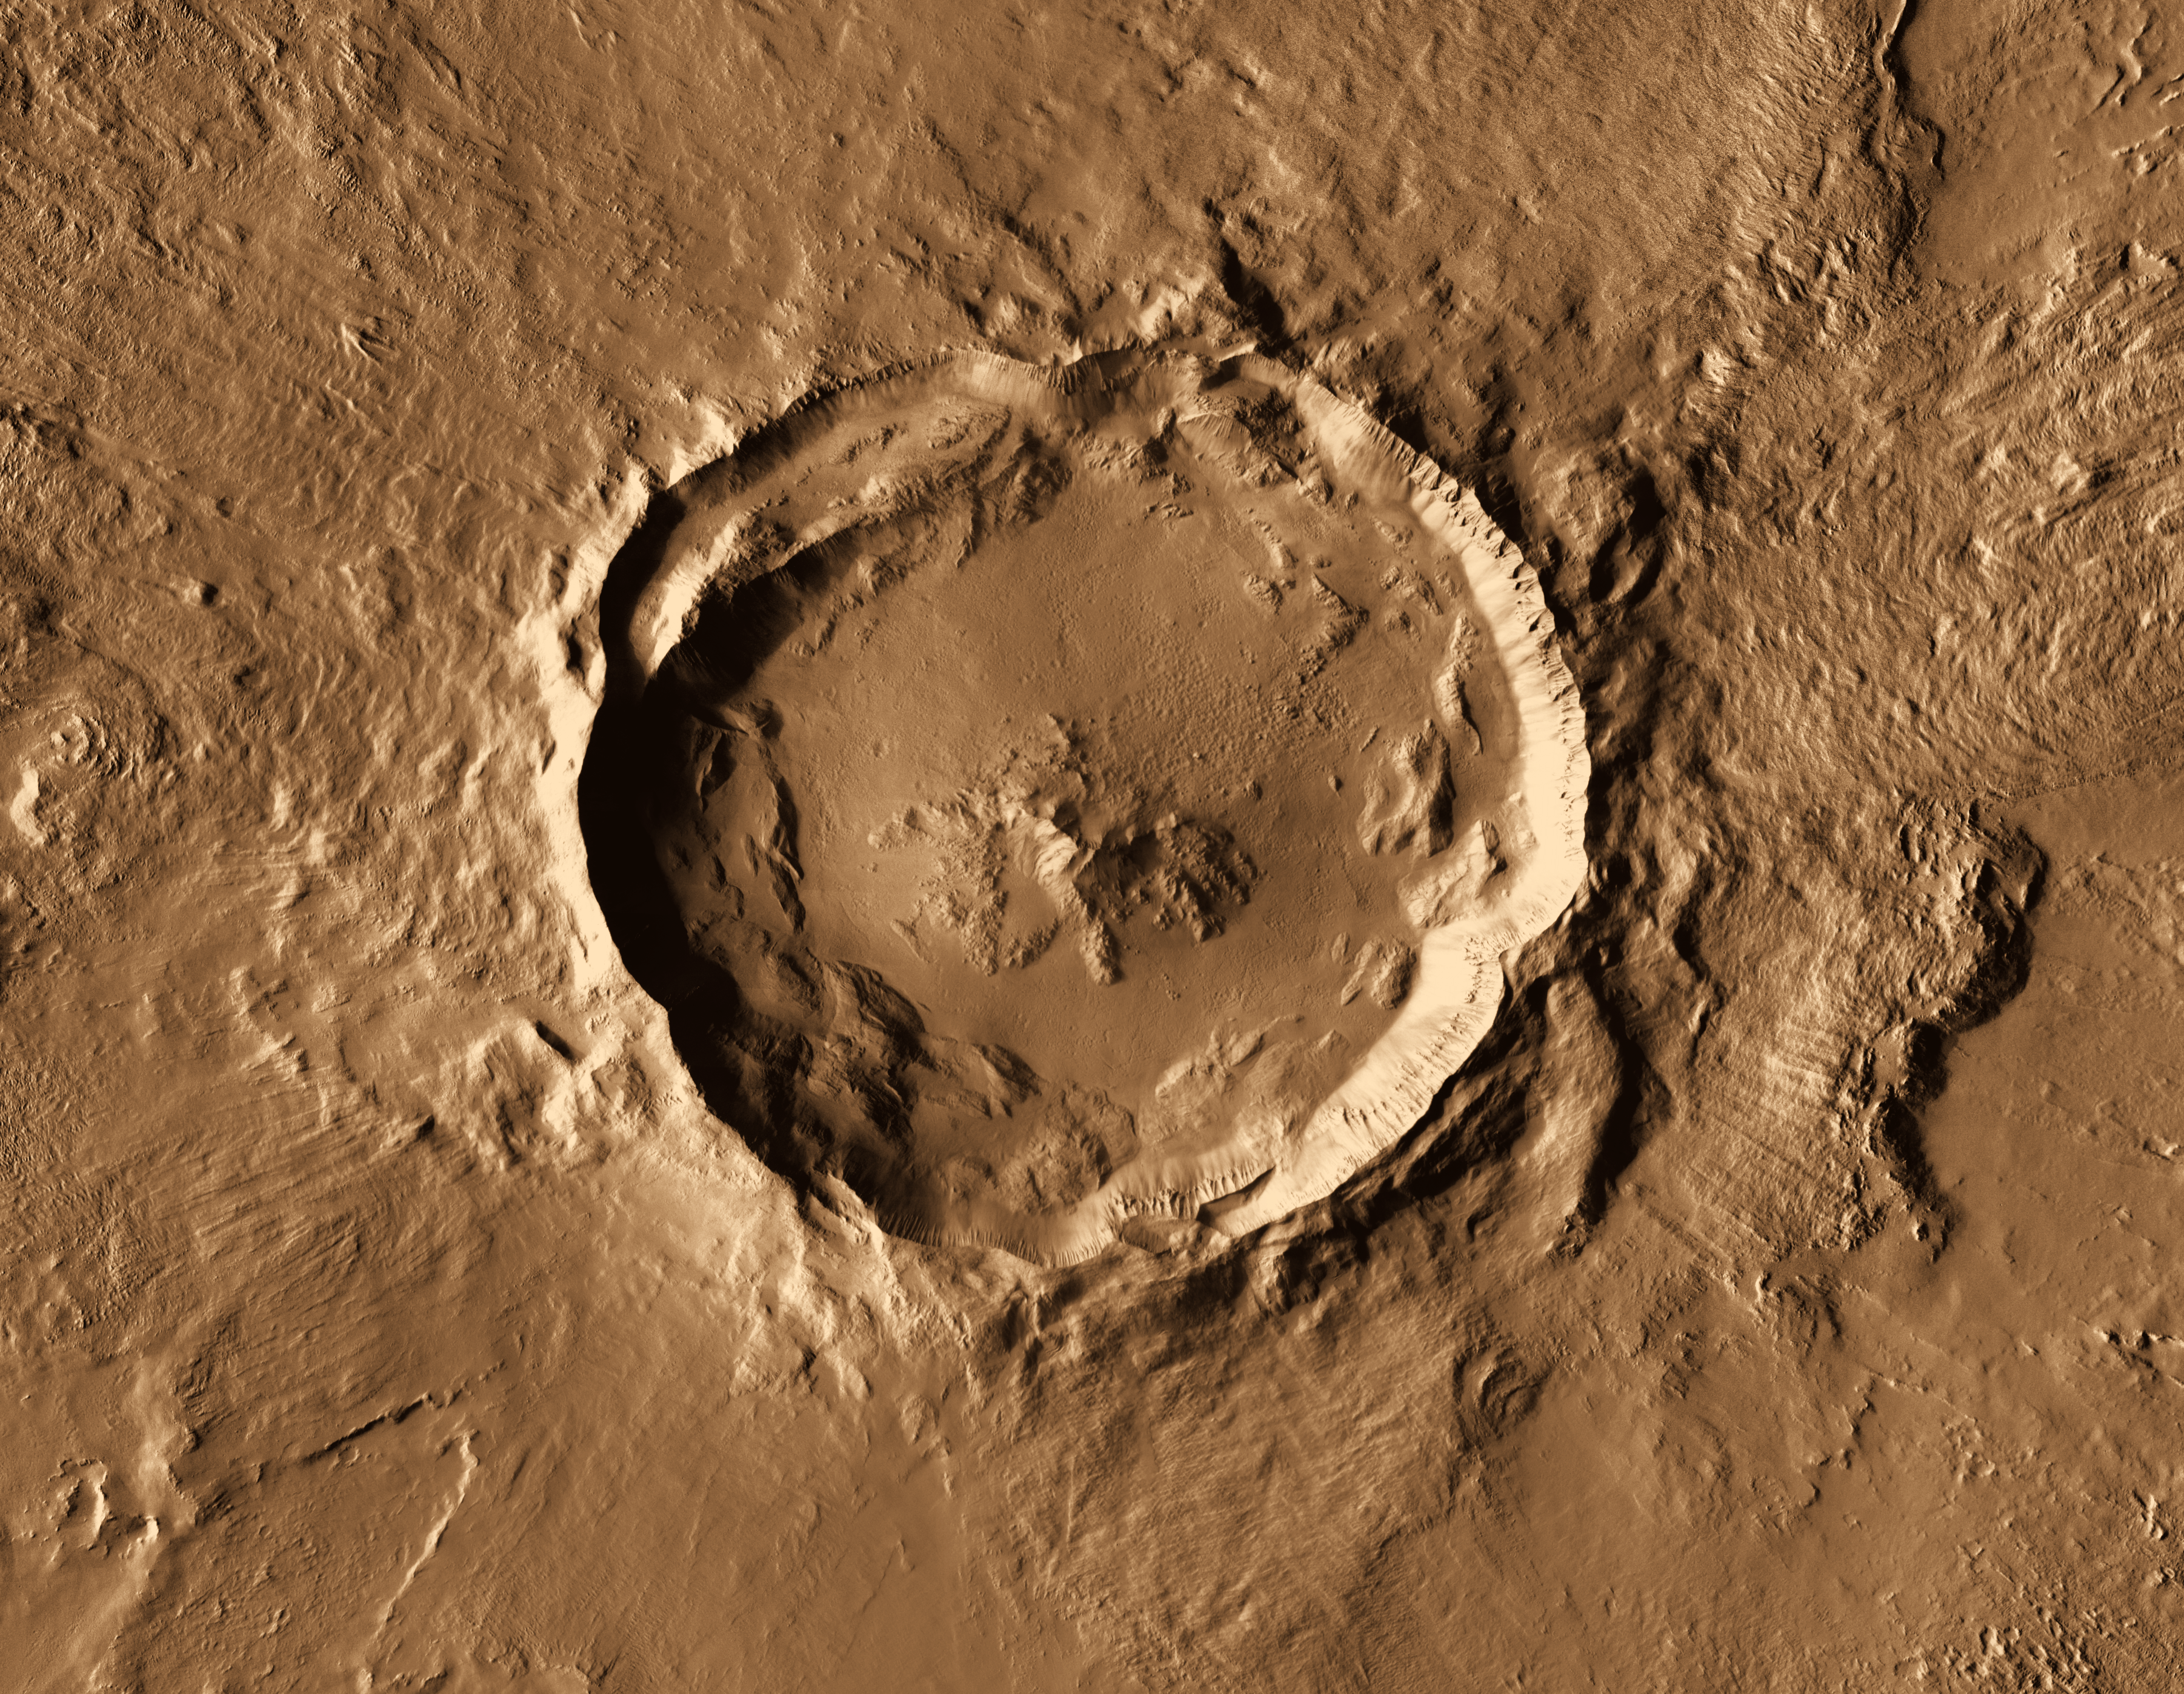
\includegraphics[width=0.45\textwidth]{../Quellen/Bilder/Tooting.png}
        \caption{Links: Topografisches Profil des Tooting-Krater, das durch den höchsten Punkt des
                Zentralbergs verläuft. Die vertikale Maßstabsverzerrung beträgt ×10. Entnommen aus \citet[1619]{Mouginis-Mark_2012}.\\
                Rechts: Foto des Tooting-Kraters. Ausschnitt von der Aufnahme der THEMIS-Mission der NASA.
                aufgerufen am 29.08.2026. URL: \url{https://themis.mars.asu.edu/files/features/043_tooting_crater/043tooting.png}}
        \label{pic:tooting}
    \end{figure}
\end{center}





\mysubsection{Entstehung}

Der Prozess der Kraterbildung lässt sich in drei Phasen unterteilen.
Das Ergebnis der Kontakt und Kompressionsphase, sowie der Aushölungsphase ist eine konkave, transiente Kraterform.
Das Ausmaß der dritten Phase, der Modifikationsphase, ist für uns interessant und von der Größe des Kraters abhängig.
Die instabile Kraterform führt bei kleineren Kratern dazu,
dass die Kraterrände hinabfallendes Gestein die Form des Kraters abflacht.
Bei größeren Kratern entsteht eine zentrale Erhebungen durch sich hebendes Gestein \citep[10]{Rae_2018}.
Solche Krater werden als komplexe Krater bezeichnet und besitzen abgesehen von Zentralbergen oder Zentralringen
häufig auch weitläufige terrassenförmige Zonen am Kraterrand, die hier nicht weiter behandelt werden sollen \ebd[].

Der Kraterradius, ab dem ein Zentralberg zu finden ist, wird größtenteils von der Größe des Himmelskörpers definiert.
So beträgt der minimale Radius auf dem Mond $\sim$15~km, auf Mars und Merkur etwa 7~km und auf der Erde $\sim$2-4~km,
abhängig von vorhandenen Gesteinsarten \ebd[12].





\mysubsection{Zentralringe}

In besonders großen Kratern wird der Zentralberg zu hoch, um stabil zu bleiben und
kollabiert zu einem Zentralring \citep[115]{Rae_2018}.
Diese ringförmigen Reliefs existieren sowohl auf anderen Himmelskörpern aus auch auf der Erde.
Der Chicxulub-Krater auf der Yucatán-Halbinsel in Mexico besitzt einen Durchmesser von etwa 180~km und
einen 400~m hohen Zentralring \citep[100]{Rae_2018}. Der $\sim$65,5 Millionen Jahre alte Krater entstand durch
den Asteroiden, welcher das Massenaussterbens am Ende der Kreidezeit verursachte und
unter Anderem zum Aussterben der Dinosaurier führte \citep[1214]{Schulte_2010}.

Der instabile Zentralberg hat nach Berechnungen seine maximale Höhe nach $\sim$200~s erreicht und
kollabierte dann zu dem heutigen Zentralring mit 80-90~km Durchmesser \citep[100, 113]{Rae_2018}.
Dessen Gestein findet sich nur zwischen 30 und 45~km entfernt von der Kratermitte \ebd[113].
Auch beweist die Existenz von kristallienen Quarzstrukuren im Zentralring ein Anheben dieses
Gesteins während der Modifikationsphase
von mehr als 2~km \ebd[102 f.].





%---------------------------------------------------------------------------------
% Äquatorialkämme


\mysection{Äquatorialkämme}
\mysubsection{Iapetus einzigartiges Gebirge}

Eines der mysteriösesten Objekte im Sonnensystem ist der Äquatorialkamm des Saturnmondes Iapetus
(siehe Abb.\ref{pic:iapetus}).
Auf Bildern der 2004 am Iapetus vorbeigeflogene Cassini-Sonde ist ein Gebirgsring am Äquator
des Mondes zu sehen \citep[1237]{Porco_2005}.
Dieser bis zu 20~km hohe Äquatorialring \ebd[1241] erstreckt sich nicht durchgehend über
mindestens 75\% des Umfangs von Iapetus \citep{Dombard_2008}.

Der Gebirgsring ist zusammen mit der Cassini-Region, einer im Vergleich zu Iapetus restlicher Oberfläche
etwa um den Faktor zehn dunklere Region \citep[1241]{Porco_2005},
eines der ältesten Merkmale des Iapetus \citep[361]{Giese_2008}.
Da er in manchen Regionen aus drei parallel verlaufenden Berggraten besteht \citep[1242]{Porco_2005},
gibt es viel Diskurs zu seiner Entstehung.



\begin{center}
    \begin{figure}
        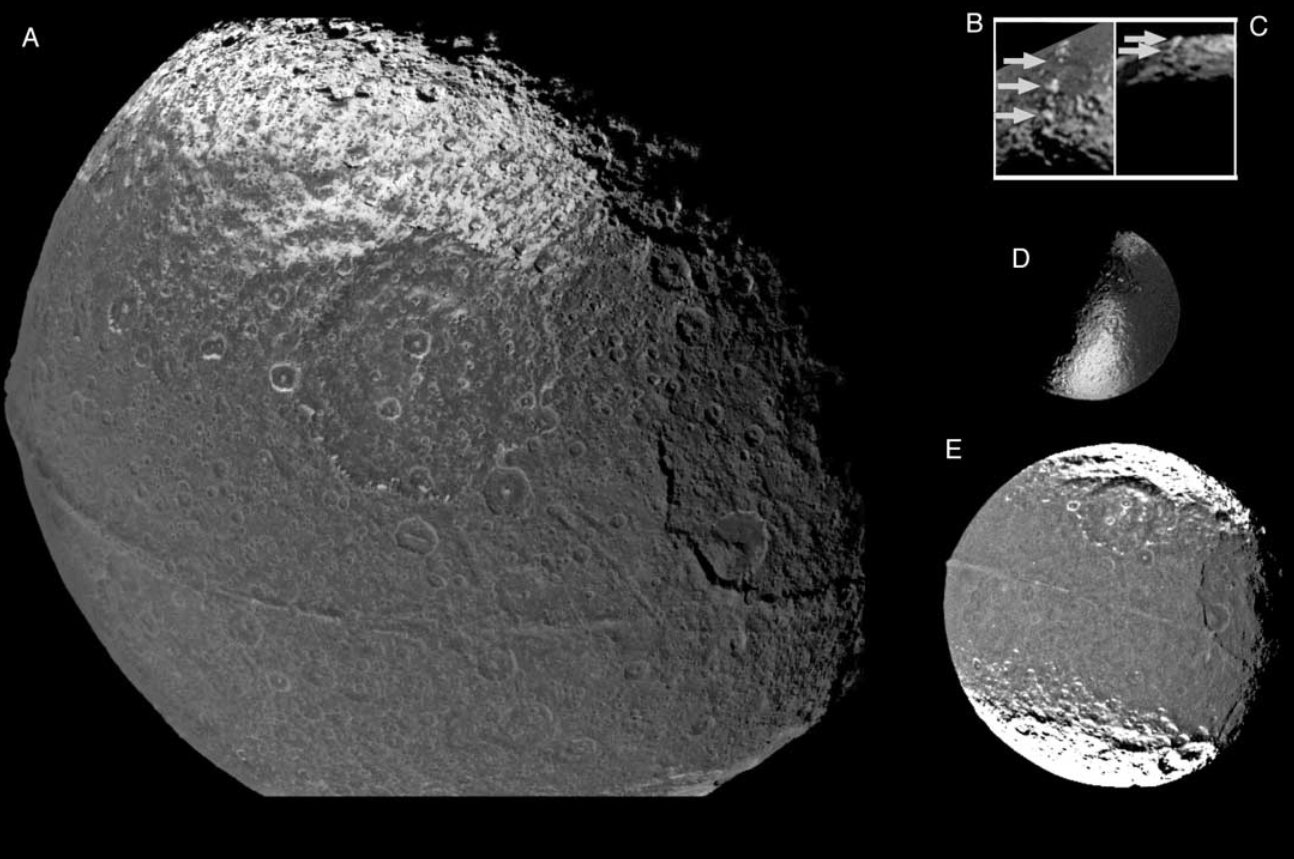
\includegraphics[width=\textwidth]{../Quellen/Bilder/Iapetus.png}
        \caption{Aufnahmen der Saturnmondes Iapetus; Entnommen aus \citet[1240]{Porco_2005}}
        \label{pic:iapetus}
    \end{figure}
\end{center}






\mysubsection{Entstehungstheorien}
Seit der Entdeckung des Äquatorialkamms von Iapetus wurden verschiedene Theorien zu seiner Entstehung aufgestellt.
Vorgestellt wurden verschiedene intrinsische und extrinsische Entstehungsmechanismen.

Intrinsische Mechanismen sind solche, dessen Ursprung auf oder in Iapetus selbst liegt.
Dazu gehören ein Verlangsamen der Rotationsgeschwindigkeit 
(siehe Kapitel \ref{subsubsec:Verlangsamen der Rotationsgeschwindigkeit des Iapetus})
und ein Aufwölben der Lithosphäre (siehe Kapitel \ref{subsubsec:Aufwölben der Lithosphäre}).

Extrinsische Mechanismen sind solche, dessen Ursprung außerhalb des Iapetus liegt.
Dazu gehört die Existenz eines uralten Ringsystems (siehe Kapitel \ref{subsubsec:Ein uraltes Ringsystem})
und die Entstehung durch einen Einschlag eines anderen Körpers auf dem Iapetus
(siehe Kapitel \ref{subsubsec:Impaktbedingte Entstehung des Äquatorialkamms}).





\mysubsubsection{Verlangsamen der Rotationsgeschwindigkeit des Iapetus}

Bereits kurz nach der Entdeckung des Iapetus wurde die Möglichkeit der Entstehung des Kamms
durch ein Verlangsamen der Rotationsgeschwindigkeit des Iapetus aufgebracht \citep[1242]{Porco_2005}.
Begründet wurde dies durch seine äquatoriale Position \ebd[].

Bei genauerer Betrachtung weißt der Iapetus eine Äquatoriale Ausbeulung vor \citep[182]{Castillo-Rogez_2007}.
Der Durchmesser von Pol zu Pol ist somit kleiner als der Durchmesser in der Äquatorebene.
Aufgrund der aktuellen Dichte und Rotationsgeschwindigkeit des Mondes sollte es eine Abweichung
von durchschnittlich $\sim$10~m zwischen diesen beiden Durchmessern geben \citep[580]{Thomas_2007}.
Die gemessene 35~km-Differenz ist in Iapetus Fall durch die Zentrifugalkraft bei einer Rotationsdauer
von $\sim$16~h zu erklären \ebd[]. Jedoch besitzt der Iapetus heute eine
Rotationsdauer von 79,33 Tagen \citep[180]{Castillo-Rogez_2007}.

Die Form des Mondes und sein Äquatorialkamm ist nach dieser Theorie durch eine hohe Rotationsgeschwindigkeit 
entstanden \ebd[182]. Damit diese durch Zentrifugalkraft stabil gehaltene Form nicht aufgrund der Verlangsamung
der Rotationsgeschwindigkeit zusammenfällt, muss die vorher dünne Lithosphäre dick genug werden um stabil genug 
zu werden um die Form des Iapetus aufrecht zu erhalten \ebd[198].

Somit folgt dem initialen Verformen des Iapetus aufgrund von Rotationsgeschwindigkeit und einer dünnen Lithosphäre
eine Phase des Abbremsens der Rotationsgeschwindigkeit mit gleichzeitiger Verdickung der Lithosphäre.
Wobei dieses Abbremsen nicht-linearer sein darf, um diesen Prozess zu erklären \ebd[].





\mysubsubsection{Ein uraltes Ringsystem}

Als alternative Entstehungstheorie zum Verlangsamen der Rotationsgeschwindigkeit
von Iapetus wurde die extrinsische Theorie eines Ringsystems vorgeschlagen.
Diese basiert auf den Funden von natürlichen Satelliten, die größere Objekte im Kuipergürtel umkreisen \citep[4]{Ip_2006}.
Das Ringsystem existiert nach dieser Theorie zu einer Zeit, wo die Oberfläche
des Iapetus weitgehend ausgehärtet ist, sodass die hinabfallenden Ringbestandteile sich nach und nach
zum heutigen Äquatorialkamm anhäufen konnten \ebd[3]. Das ursprüngliche System müsste eine
Masse von $\sim$0,1\% von der des Iapetus besitzen \ebd[].

Das Existieren eines Ringsystems wird von der Größe des Iapetus begünstigt.
Denn der Iapetus besitzt eine vergleichsweise Hill-Sphäre, also der Bereich um einen Himmelskörper,
in dem seine Anziehungskraft gegenüber anderen Körpern überwiegt \ebd[2].

Die einzelnen Ringobjekte müssen auf ihrer Bahn abgebremst werden, um auf den Mond zu fallen.
Dies geschieht einerseits durch Kollisionen zwischen den Objekten und andererseits durch die Annahme,
dass der Iapetus zu der Zeit eine dünnen Atmosphäre besaß, welche die Objekte durch Reibung abbremst \ebd[3].

Alle anderen Monde des Saturn besitzen eine Inklination, also Bahnneigung, von $\sim$0\degree \ebd[4].
Die Inklination des Iapetus liegt währenddessen bei $\sim$7,49\degree \citep[180]{Castillo-Rogez_2007}.
\citeauthor{Ip_2006} bringt die Möglichkeit einer Kollision mit einem anderen Himmelskörper als Hintergrund
der Inklinationsanomalie und des Ringsystems auf \ebd[]. Demnach ist der Ring nicht wie in seiner Theorie
ein Überrest der Entstehung des Iapetus sondern impaktgeneriert ist. Diese Beobachtung führe zur weiteren Untersuchung
dieser Möglichkeit (siehe Kapitel \ref{subsubsec:Impaktbedingte Entstehung des Äquatorialkamms}).




\mysubsubsection{Aufwölben der Lithosphäre}

Um die Schwächen der vorangegangenen Theorien zu umgehen, wurde ein Aufwölben der Lithosphäre,
also der äußersten Gesteinshülle, als Entstehungsmechanismus in Betracht gezogen.
So besitzt der Äquatorialkamm eine komplexe, sich über seine Länge ändernde Form \citep[365]{Giese_2008}.
Die an einigen Stellen vorkommenden flachen Bergspitzen mit scharfen Kanten an ihren Seiten sind
nicht durch die Theorie eines Ringsystems erklärbar (siehe Kapitel \ref{subsubsec:Ein uraltes Ringsystem}) \ebd[].
Auch sprechen Ausgedehnte parallel zum Kamm verlaufende Senken für ein verbiegen der Lithosphäre \ebd[364].

Des Weiteren wäre bei einem aus kleinen Ringbestandteilen bestehendem Kamm eine Steigung
nahe der maximalen Steigung, wo ein solcher Berghang stabil bleiben würde, zu erwarten \ebd[].
Dies ist gerade bei den unteren Hängen nicht der Fall und die geringe Steigung spricht eher 
für einen intrinsischen Mechanismus \ebd[].

Am wahrscheinlichsten ist ein zwei-Zellen-Konvektionsmuster, welches tiefliegendes Gestein Richtung
Oberfläche schiebt und die Lithosphäre zu einem äquatoriellen Bergsystem aufwölbt \citep[64, 65, 68]{Czechowski_2008}.
Angetrieben wird dieser Mechanismus von Abwärme durch radioaktiven Zerfall im Inneren des Iapetus \ebd[64].




\mysubsubsection{Impaktbedingte Entstehung des Äquatorialkamms}

Als Erweiterung der Theorie von \citeauthor{Ip_2006} (siehe Kapitel \ref{subsubsec:Ein uraltes Ringsystem})









\mysubsubsection{Daphnis, Atlas und kp wie der hieß}








%---------------------------------------------------------------------------------
% Vulkanismus


\mysection{Vulkane}

Vulkanismus ist ein relativ weit verbreitetes Phänomen in unserem Sonnensystem.
Nicht nur gibt es aktiven Vulkanismus auf der Erde
(siehe Kapitel \ref{subsec:Vulkanismus auf der Erde}),
sondern auch auf der Venus und dem Jupitermond Io
(siehe Kapitel\ref{subsec:Vulkanismus auf dem Io}) \citep[687]{Sigurdsson_2015}.
Auf dem Mars existieren die höchsten Vulkane des Sonnensystems, wie der Olympus Mons
(siehe Kapitel \ref{subsec:Vulkanismus auf dem Mars}) \ebd[],
und die Venus zeigt Anzeichen von aktuellen vulkanischen Prozessen
(siehe Kapitel \ref{subsec:Vulkanismus auf der Venus}).

Auch zeugen große vulkanisch Ebenen auf unserem Mond und dem Merkur von einer
aktiven geologischen Frühgeschichte dieser Himmelskörper
(siehe Kapitel \ref{subsec:Basaltebenen auf Mond und Merkur}) \citep[687]{Sigurdsson_2015}.




\mysubsection{Vulkanismus auf der Erde}

Der Vulkanismus auf der Erde beschäftigt die Menschen seit ihrer Entdeckung und wurde inzwischen
umfassend erforscht und verstanden.

An den Orten im äußeren Erdmantel, an dem sich Hitze anstaut, sogenannten Hotspots,
schmilzt das Gestein mit der geringsten
Schmelztemperatur und sammelt sich in größeren Reservoir \citep{USGS_Volcanism}.
Überdruck in diesen Kammern drückt das geschmolzene Gestein, Magma genannt, durch strukturell
schwache Zonen und Risse im Gestein bis an die Oberfläche \ebd[].
Sobald die Magma an die Oberfläche tritt wird sie Lava genannt und es handelt sich um eine Eruption.
Diese kann entweder explosiv unter Bildung von Lavafontänen oder nicht-explosiv als \glqq herausfließen\grqq aus
dem Gestein geschehen \ebd[].

Der Vulkan selbst bildet sich aus diesem sich nach und nach anhäufendem Gestein \ebd[].
Die Inselkette Hawaii ist beispielsweise vulkanischen Ursprungs und beherbergt
Vulkane, die sich bis zu 9~km über den Meeresboden erstrecken \citep{Fraknoi_2022}.






\mysubsection{Basaltebenen auf Mond und Merkur}









\mysubsection{Vulkanismus auf der Venus}

Die Venus ist in etwa so groß wie die Erde und besitzt durch ihren Aufbau und Stärke der
Gravitation die Voraussetzungen für lange anhaltenden Vulkanismus \citep[67]{Ivanov_2013}.
Aufgrund dieser Eigenschaften und ihrer dicken Atmosphäre als Schwesterplanet der Erde bezeichnet,
ist die Venus dennoch sehr lebensunfreundlich. Die Oberflächentemperatur beträgt 460\celsius, weshalb
heutzutage keine Wasser mehr existiert und die unter einem Druck von 90~bar stehende Atmosphäre und
Oberfläche sehr trocken sind \citep[606]{Smrekar_2010}.
Hierdurch sind auch für den Vulkanismus vollständig andere Bedingungen gegeben.

Rund 80\% der venusischen Oberfläche bestehen aus vulkanischem Material \ebd[67].
Dies liegt an einer globalen Oberflächenerneuerung, einem starken vulkanischen Event, bei dem innerhalb
der letzten 100 Millionen Jahre fast die gesamte Oberfläche der Venus erneuert wurde \citep[42]{Nimmo_1998}.
Ob es sich um ein kurzes Extremereignis oder einen langen Prozess handelte ist unbekannt \ebd[40].
Bekannt ist, dass die geologische Aktivität der Venus seitdem zurückgegangen ist \ebd[].

Vulkanische Ebenen sind die weiterbreitetsten vulkanischen Strukturen auf der Venus \citep[68]{Ivanov_2013}.
Auch Schildvulkane sind bekannt, die im Vergleich zur Erde deutlich größer und mit einer Hangsteigung von
<3\degree auch flacher sind \citep[2]{Mason_2025}.
Der Ozza Mons zeigt genau diese geringe Steigung. Er ist mit 7,5~km ein mittelhoher Vulkan der Venus, aber
1000~x~800~km breit \ebd[12].
Der Maat Mons ist der doppelten Höhe des Ozza Mons der höchste Vulkan der Venus, allerdings weniger breit \ebd[13].

Der Grund für das große Ausmaß der Schildvulkane ist die Abwesenheit von starker Plattentektonik,
wie der auf der Erde \citep[2f.]{Nimmo_1998}.
Durch die weniger dichte Lithosphäre wird Subduction, also ein Abtauchen von Teilen der Lithosphäre unter
Anderen Teilen, verhindert und die Lithosphäre ist weniger Mobil \ebd[40].
Somit ergibt sich ein sich langsam über einen stationären Hotspot verschiebender Vulkanismus 
mit vergleichsweise großen Schildvulkanen \parencites[17]{Mason_2025}[2f.]{Nimmo_1998}.

Die Venus gilt auch aktuell noch als vulkanisch aktiver Himmelskörper \citep[607]{Smrekar_2010}.
Durch Aufnahmen im Infrarotbereich durch die Venus Express Sonde konnten verschiedene Bereiche mit hoher
Emission von Infrarotstrahlung indentifiziert werden \ebd[605, 606].
Da einige dieser Orte Vulkane, wie der Idunn Mons oder Hathor Mons sind \ebd[606], ist eine rezente vulkanische
Aktivität auf der Venus sehr wahrscheinlich. Auch zeigt ein relativ junker Gesteinsstrom in der Themis Region
hohe Emissionsraten, was diese Annahme weiter untermauert \ebd[].






\begin{center}
    [ coronae (ivanov,mason)]
\end{center}





\mysubsection{Vulkanismus auf dem Mars}








\mysubsection{Vulkanismus auf dem Io}











%---------------------------------------------------------------------------------
% Verzeichnisse

\newpage
\pagenumbering{Roman}
\setcounter{page}{2}

\addcontentsline{toc}{section}{Abbildungs- und Literaturverzeichnis}

\listoffigures
\printbibliography[title={Literaturverzeichnis}]



%---------------------------------------------------------------------------------
% Eigenständigkeit

\StartBackground
\pagestyle{empty}
\pagenumbering{gobble}

\newpage
\noindent{\fontsize{14pt}{16pt}\selectfont \textbf{Erklärung des Verfassers}}\\[0.5cm]
Hiermit erkläre ich, dass ich die vorliegende Arbeit selbstständig angefertigt,
keine anderen als die angegebenen Hilfsmittel benutzt und die Stellen der Facharbeit,
die im Wortlaut oder im wesentlichen Inhalt aus anderen Werken oder dem Internet entnommen wurden,
mit genauer Quellenangabe kenntlich gemacht habe.\\[0.5cm]

\noindent Verfasser:\quad Julian Luke Mawill Baden\\[0.8cm]

\hspace{1cm} \stackunder[4pt]{\rule{4.5cm}{0.6pt}}{\makebox[4.5cm]{Ort und Datum}}
\hspace{2cm} \stackunder[4pt]{\rule{5.5cm}{0.6pt}}{\makebox[5.5cm]{handschriftliche Unterschrift}}



\end{document}